\section{Linking the WöWö}

A number of online dictionaries for Low German are available, but usually not under permissive licenses. As a result, we focus on the \emph{WöWö} dictionary as our primary dataset, and do currently not provide Linked Data editions of other Low German dictionaries. However, these are accessible online, usually with URIs identifying the respective lemma, and we use only \emph{this information} (the existence of a lemma and the assignment of a particular URL) to create a machine-readable `entry point' (i.e., an index) in RDF. As we do not use any specific information from the dictionaries other than the existence of a lemma, we assume that this information does not meet the threshold of originality legally required for copyright to apply \citet{Margoni2016},
so that these LOD indices to other Low German dictionaries can be published as addenda to the \emph{WöWö} dataset regardless of the licensing situation of the full data sets. However, should these respective resources be ever served as Linked Data or be made accessible under a more permissive license, the information from the indices/links we provide can be seamlessly integrated into the respective dictionaries.

\subsection{External Datasets}

The dictionaries that we link with the \emph{WöWö} are perfect silos, in the sense that they are isolated from any other content available on the web. Yet, this does not mean that they do not contain links. In fact, \emph{several} of the existing platforms have been \emph{designed} to provide inter-dialectal links, resp., links between different dictionaries, but they only provide links \emph{within} the respective ecosystem, whereas we pursue an open, extensible approach capable of integrating \emph{any} piece of information accessible on the web. 

\begin{itemize}
\item The Trier Wörterbuchnetz\footnote{\url{https://woerterbuchnetz.de/}} is an online platform that provides online access to dictionaries of historical and regional vernaculars, predominantly from Germany, including dictionaries for historical stages and dialects of German. Among Latin, Ladin, Uighur and Russian, it also comprises a major dictionary of the Westphalian dialect of Low German. %Aside from basic search, it provides links between languages of related varieties. This includes bibliographical references, but also HTML hyperlinks. 
Overall, the Wörterbuchnetz builds on mature XML technologies to provide human-readable content, and there also is an API that can be used to retrieve a lemma list (but not the content itself). Within the Wörterbuchnetz, hyperlinks are limited to resources provided by the Wörterbuchnetz itself -- and at the moment, none of these are concerned with Low German, %However, a dictionary of Mecklenburgian is currently in the process of integration,\footnote{\url{https://www.germanistik.uni-rostock.de/personen/professuren/prof-dr-andreas-bieberstedt/projekte-und-forschungsschwerpunkte/wossidlo-teuchert-online/}}
but if these should ever emerge, our linking technology may be trivially expanded to them as well as to other Wörterbuchnetz data, if a phonological mapping can be established.

\item The Digitales Wörterbuch Niederdeutsch (DWN)\footnote{\url{https://www.niederdeutsche-literatur.de/dwn/}} by Peter Hansen is a website that provides access to a `basis' Low German dictionary (adopting spelling rules developed for North Low Saxon), a dictionary for Mecklenburgian-Western Pomeranian as well as custom dictionaries for selected authors (Klaus Groth, Fritz Reuter and John-Brinckman Wörterbuch). Each dictionary comes with its own search dialog, and little is known about the technical details, as only a human-readable HTML rendering is accessible. Within each dictionary, lemmata are linked across these datasets with HTML links. We presume that this uses standard SQL technology. Again, no links to external resources are being provided.
As the content is copyright-protected, we decided to work only with the Reuter dictionary based on \citep{muller1904reuter}, as this goes back to a print dictionary in the public domain. We did not exploit the interdialectal links provided by the DWN, nor did we use any of its original content.
\item Plattmakers\footnote{
    \url{https://plattmakers.de/de}
} is an online aggregate dictionary with 22.000 entries provided in a single, searchable database, and developed by Marcus Buck. It provides its content in human-readable fashion, and individual entries are equipped with maps and links to the source literature. Plattmakers is a private website, but some details about its implementation are provided,\footnote{\url{https://plattmakers.de/de/faq}} indicating that it is based on a relational database backend, and supported by automated normalization routines similar to those described below. Unlike DWN and Wörterbuchnetz, Plattmakers lemma URLs provide machine-readable metadata in JSON-LD, so that its content \emph{can} be processed and evaluated in conjunction with \emph{WöWö} information. At the same time, it is copyright-protected, so that we do not work with any Plattmakers information except for URL and lemma form. %Unlike DWN and Wörterbuchnetz, Plattmakers is a private initiative not supported by any academic institution, and some of its more recent content seem to be crowd-sourced and not to meet scientific standards. Yet, it is seems to be more usable than either DWN or Wörterbuchnetz, because it provides direct, interdialectal search capabilities across all dictionaries it covers. 
\ign{
We assume that our linking implementation partially replicates functionalities of the Plattmakers backend, but that we provide an added value in extending these to content not covered by Plattmakers, and in particular, to other dictionaries maintained by providers supported by or collaborating with academic institutions such as Wörterbuchnetz and DWN, so that conjoint queries over their aggregate content are capable of providing more detailed (or, more substantiated) information than queries over Plattmakers content alone.
}\end{itemize}

\noindent
Overall, we link five online dictionaries, covering the main branches of modern Low German, each identified with language combine ISO 639-2/-3 codes with Glottolog identifiers:\footnote{\url{https://glottolog.org/}} in the BCP47 `private use' section: 

\begin{description}
\item[Plattmakers] (for North Low Saxon/North Hanoveranian, \code{nds-x-nort3307}).
\item[WWB] Westfälisches Wörterbuch from Wörterbuchnetz (for Westphalian, \code{wep}).
\item[Twents] Twents Woordenboek by Goaitsen van der Vliet (2025), available for online search under \url{https://twentswoordenboek.nl} and published under CC BY-NC-SA (\code{twt}, a Dutch Westphalian dialect).
\item[Reuter] dictionary from DWN (for Mecklenburgian, resp., East Low German in Germany, \code{nds-x-meck1239})
\item[Plautdietsch] (Mennonite Low German) dictionary by Herman Rempel and the Mennonite Literary Society (1984-1995), \url{mennolink.org} (1998-2006), and Eugene Reimer (2006-2007), published under CC BY-SA\footnote{\url{https://ereimer.net/plautdietsch/pddefns.htm}} (for emmigrant varieties of East Low German, \code{pdt}). 
\end{description}

\subsection{Data Retrieval and Processing}

Creating an LOD index for a dictionary typically requires to retrieve a list of lemmas, e.g., by crawling its content in order to extract lemma forms and lemma URL which are then stored in a TSV file. 
From these initial TSV files, we then create an extended TSV file that adds two additional columns, the lemma form in \emph{WöWö} (for verification), and the \emph{WöWö} URL (for the actual linking). All the dictionaries that \emph{WöWö} will be linked with comprise form-level information, only, linking is grounded on \emph{formal agreement} only, so that in most cases, there are many-to-many relationships between dictionary lemmas and \emph{WöWö} entries (cf. Fig. \ref{fig-twents-woewoe}).

This data is diverse in phonology and orthography, so that formal linking must not rely on mere identity. Instead, we use Finite State Transducers to generate hypothetical normalizations against one specific variety of Low German and then generate candidate links for lemmas from different dictionaries for which identical forms are generated. We normalize towards North Markian, an East Low German variety that resembles the North Low Saxon dialects of \emph{WöWö} and Plattmakers in exhibiting both a reduced inventory of diphthongs and the systematic dropping of unstressed Middle Low German \word{e} (apocope, syncope). The mapping is implemented with the Stuttgart FST library \cite[SFST]{schmid2006programming}, using the sound correspondences established by Pfaff (1898)\nocite{pfaff1898vocale}, Teuchert (1907)\nocite{teuchert1907mundart} and Mackel (1905)\nocite{mackel1905mundart}. As for the effort required to implement a mapping, this normally took about a day per dataset. Low German dialects don't deviate much in their consonants, but coonlynsiderably both in their vowel inventories and the spelling of vowels. The normalization is not exposed to the user, but used internally, only: We predict a candidate link for every pair of lemmas that have at least one normalized form in common.

\begin{figure}
    \flushleft
    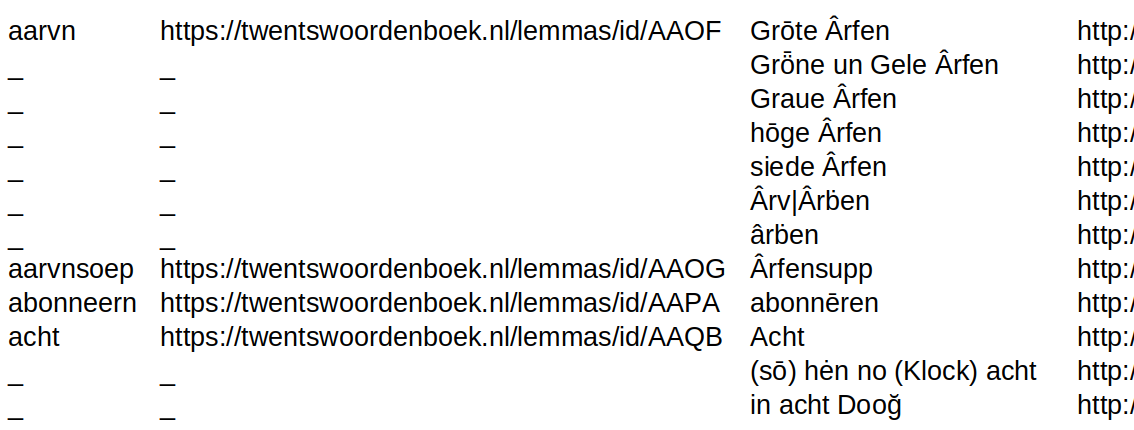
\includegraphics[width=1\linewidth]{img/tsv-linked.png}
    \caption{Linked TSV file except, Twents (left) to \emph{WöWö} (right)}
    \label{fig-twents-woewoe}
\end{figure}

For the RDF export, we calculate the confidence of a link $\langle x,y\rangle$ as the harmonic mean between the linking probabilities $P(x|y)$ and $P(y|x)$, with $P(x|y)$ and $P(y|x)$  estimated from the the total of many-to-many candidate links for the lemmas $x$ and $y$, respectively. In the RDF export, we only include the most probable links. \ign{
    If there is more than one, we return the \emph{WöWö} lemma with the lowest Levenshtein distance. If there is still more than one, we return the shortest \emph{WöWö} lemma. If there is still more than one, we return the lexicographical first lemma.\footnote{
        The converter has a flag to return all possible links, along with their confidence, but this is disabled by default.
    }
}

\subsection{RDF Representation}

In the RDF export, we only include the most confident link, by default. For any given link $\langle x,y\rangle$, the confidence score $c(x,y)$ is calculated as $c(x,y)=2 \frac{P(x|y) P(y|x)}{P(x|y) + P(y|x)}$. If more than one match with the same score is found, we return the one with lowest Levenshtein distance. If this is not umambiguous, we return the shortest target URL in order to create a bias against partial matches. For every external dictionary, we create one lexical entry per source URL, and provide the lemma form as its canonical form. These lexical entries are then linked with \emph{WöWö} URLs.

We produce linkings in two different flavours. The condensed format only conveys a \onto{lexinfo:geographicalVariant} link between two lexical entries.\ign{
\footnote{
    `Geographical variant' is not a perfect term to describe the cross-dialectal relation between individual lexical entries, because this implies that both variants are, in fact, different. However, in many cases they are not, or their differences are merely orthographic. Better suited would be a relation that can be applied to lexical entries that are either equivalent, (virtually) identical or deviant. 
        Although more appealing from its name, we decided to not resort to \onto{lexinfo:approximate}, because it's a sense relation, not a relation induced by forms ... the sense link is unconfirmed and we don't have machine-readable senses for any dictionary other than the \emph{WöWö}.
    }
} % ign
This compact format is well-suited for downstream applications where only the link itself is processed, but it omits provenance and confidence information. Unlike the reified data described below, this is also OWL2/DL-compliant. 

As there is no manual quality control involved here and the automated linking procedure creates many $n$:$m$ correspondences, it is, however, preferred to provide the confidence scores, as well, for which we adopt a reified representation inspired by \citet{gillis2023refinement}, with a \code{vartrans:LexicalRelation} object that \code{vartrans:relates} an external lexical entry with a lexical entry from \emph{WöWö} and that uses \code{lexinfo:category} to indicate the type the of relation. There are, however, no exactly corresponding concepts in lexinfo to indicate the type of relation, so that, instead of an individual, we resort to \onto{lexinfo:geographicalVariant}, again. However, this is an object property, not an individual, the resulting data is thus propelled into the semantic space of OWL2/Full.
Every reified link is complemented with a numerical confidence score. Due to the lack of a standard vocabulary for confidence scores in RDF or LexInfo, we adopt \onto{rdf:value} for the purpose, but this is semantically underspecified. %We would recommend to create a designated LexInfo property, say, \onto{lexinfo:confidence}.

For linking WöWö \word{Ool} with the Twents dictionary, we arrive at the graph in Fig.\ \ref{fig-links}. The lexical entry \onto{:Ool} is the \emph{WöWö} lexical entry, the individual links are formally associated with a dataset object, like the individual dictionary entries are associated with their source URL that is defined as a \onto{lime:Lexicon}. However, as we only provide a shallow wrapper around the original source document, and because the URLs will not resolve to machine-readable information anyway, we bundle both linking information and the lexical entries drawn from \url{https://twentswoordenboek.nl} in a single file.

\begin{figure}
    \centering
    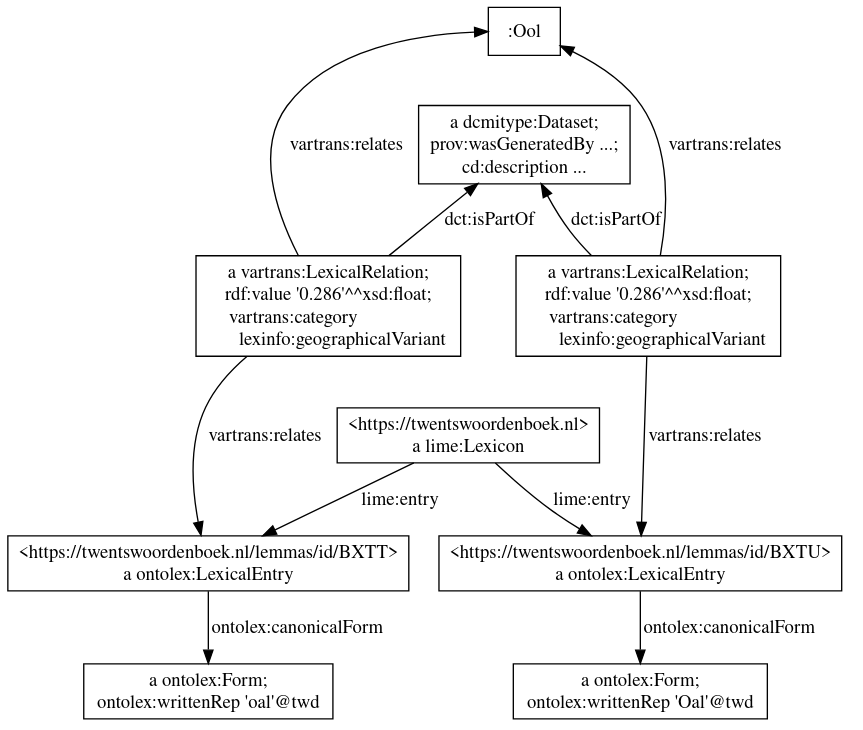
\includegraphics[width=1.05\linewidth]{img/links-vis.png}
    \caption{Reified \onto{lexinfo:geographicalVariant} links between \emph{WöWö} \word{Ool} `eal' and Twents dictionary}
    \label{fig-links}
\end{figure}

%% Dot source
% digraph G {
% 
%  ool -> bxtt_link [label=" vartrans:relates", dir=back]
%  ool -> bxtu_link [label=" vartrans:relates", dir=back]
%  ool -> ds[style=invis]
%  ool [label=":Ool",shape=box]
% 
%  ds -> bxtt_link[dir=back, label="dct:isPartOf"]
%  ds -> bxtu_link[dir=back, label="dct:isPartOf"]
% ds[label="a dcmitype:Dataset;\nprov:wasGeneratedBy ...;\ncd:description ...", shape=box]
% 
% twents[label="<https://twentswoordenboek.nl>\n a lime:Lexicon", shape=box]
% twents->bxtt[label="lime:entry"]
% twents->bxtu[label="lime:entry"]
% 
%  bxtt_link[label="a vartrans:LexicalRelation; \nrdf:value '0.286'^^xsd:float;\nvartrans:category               \n       lexinfo:geographicalVariant", shape=box]
%  bxtu_link[label="a vartrans:LexicalRelation; \nrdf:value '0.286'^^xsd:float;\nvartrans:category               \n       lexinfo:geographicalVariant", shape=box]
% 
% bxtt_link->twents[style=invis]
% 
%  bxtt_link ->  bxtt [label=" vartrans:relates",constrains=false]
%  bxtu_link ->  bxtu [label=" vartrans:relates"]
% 
%  bxtt -> oal_twd [label=" ontolex:canonicalForm"]
%  bxtt [label="<https://twentswoordenboek.nl/lemmas/id/BXTT>\n a ontolex:LexicalEntry", shape=box]
%  oal_twd [label="a ontolex:Form;\nontolex:writtenRep 'oal'@twd", shape=box]
% 
%  bxtu -> Oal_twd [label=" ontolex:canonicalForm"]
%  bxtu [label="<https://twentswoordenboek.nl/lemmas/id/BXTU>\n a ontolex:LexicalEntry", shape=box]
%  Oal_twd [label="a ontolex:Form;\nontolex:writtenRep 'Oal'@twd", shape=box]
% 
% }

\ign{ % we have this in summary
    Another apparent gap in LexInfo is the lack of a counterpart of translation set for lexico-semantic relations other than translation. In its place, we resort to \url{http://purl.org/dc/dcmitype/Dataset}. This is needed to store provenance information (which otherwise needs to be repeated for every lexical link). Every lexical-semantic relation is linked by \onto{dct:isPartOf}.
}